% !TEX root = C:\Users\Jan\Documents\dev\Risk-Measurement-Framework\masterthesis_tex\masterthesis_main.tex
\section{Implementation}
\label{sec:implementation}

The technical RMF uses Python 3.7 as the programming language and ART as the basis. Beside the attacks given by the ART, there is a function from the technical RMF to execute individual attacks. This technical RMF should be used a step ahead of using the framework of Schwerdtner et al.

\subsection{Structure of the RMF}

\subsubsection*{Directory tree}

The RMF is structured as follows:

\dirtree{%
.1 rmf/.
.2 attacks/.
.3 art/.
.4 backdoors.py.
.2 backdoors/.
.3 png-Files.
.2 measurement/.
.3 monitoring.py.
.2 metrics/.
.3 log.py.
.2 visualizations/.
.3 plot.py.
.2 log\_file.log.
.2 case\_study.py.
}

\subsection{Implement the risk indicatiors}

The risk indicators are the main part for the risk measurement. Therefore the risk indicators are used through the complete risk measurement. Every risk indicator is implemented as an own function in the RMF. This makes it possible to measure the risk indicator values at every step during the ML model training. The goal is to use measure the risk indicator values with the original training data and the manipulated training data.

\subsection{Using ART as the basis for the technical framework}

The ART implemented two backdoor attacks which will be explained in \ref{sec:backdoors_art}. Since art is an open-source technical framework, the two backdoor attacks can also be used as a basis for simplifying the implementation of other attacks.

\subsection{Implementing backdoor attacks}

The following three attacks are all based on the ART and represent white-box and black-box attacks and both targeted and untargeted attacks. These attacks are used to measure the extent of damage and the types of attack help to measure the attackers knowledge.

\subsubsection*{Backdoor attacks from the ART}
\label{sec:backdoors_art}

All backdoor attacks use the \textit{PoisoningAttackBackdoor} class which expects a pattern argument. The pattern is a picture which is for the poisoned images in the training data. The pattern must be implemented before training and choose a random selection of images. This is implemented in the RMF as follows:

\begin{lstlisting}
  n_train = np.shape(x)[0]
  num_selection = num_of_rand_images
  random_selection = np.random.choice(n_train, num_selection)
  x = x[random_selection]
  y = y[random_selection]
\end{lstlisting}

Then the arguments $x$ and $y$ are passed to the poisoning function from the ART. $x$ and $y$ are parameters which the function expects when calling it. Appendix \ref{sec:frame_func} describe the functions and parameters. Further it is important that the shape of the images from the training data are \textit{N, H, W, C} or \textit{N, C, H, W}. $N$ is the number of images in the batch, $H$ is the image height, $W$ is the image width, and $C$ is the channel number of an image such as grayscale or RGB. After adding a backdoor as a pattern to the random images, the poisoned images are replaced back to the training data. These poisoned images are saved in a different folder to check if the images are missclassified after or while testing the ML model.\\

The first attack uses the \textit{PoisoningAttackBackdoor} class without any other backdoor classes from the ART. This attack which bases on Gu et al. \cite{DBLP:journals/corr/abs-1708-06733} is a black-box attack which is untargeted. In the RMF it uses a pattern backdoor which Figure \ref{fig:original_example} and Figure \ref{fig:poisoned_example} show as the difference between the original and the poisoned image. The goal of this attack is to change the original label to a random other label. This attack can be executed without any information because it is not important which training data the ML model use and what ML model is used for the training itself.

\begin{figure}[!tbp]
  \centering
  \begin{minipage}[b]{0.4\textwidth}
    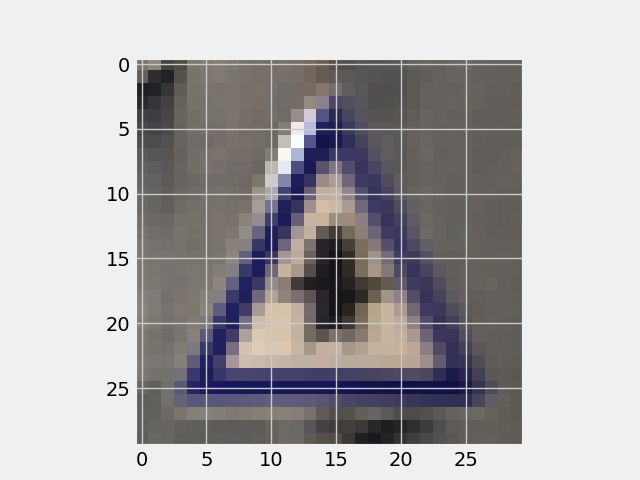
\includegraphics[width=8cm]{pictures/original_example.png}
    \caption{Street sign without a backdoor pattern with the label \textit{Right-of-way at intersection}}
    \label{fig:original_example}
  \end{minipage}
  \hfill
  \begin{minipage}[b]{0.4\textwidth}
    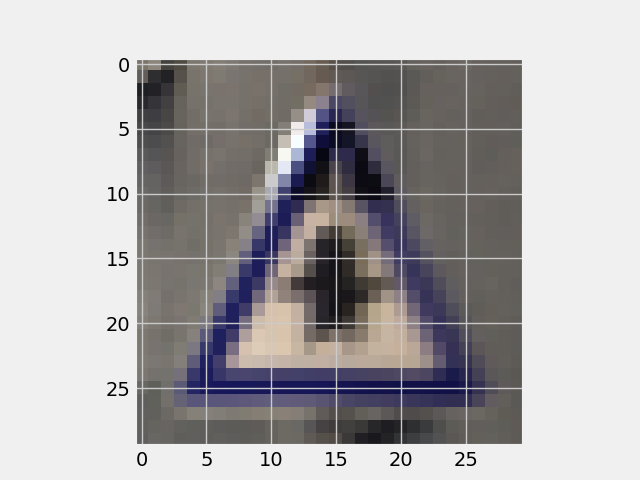
\includegraphics[width=8cm]{pictures/poisoned_example.png}
    \caption{Street sign with a backdoor pattern but still with the original label \textit{Right-of-way at intersection}}
    \label{fig:poisoned_example}
  \end{minipage}
\end{figure}

After poisoning the images these image need be copied back into the original training data. Before this can be done the poisoned data must replace the original training data which contain no backdoor. When the RMF take the random original images, it save them into a temporary variable and then delete the images from the original training data. The next step is the poisoning while the poisoned data and the original training data need the same shape and dimension which make it possible to copy the poisoned images. As mentioned before the poisoning function takes only two specific shapes which make it easy to have the same shape in the original training data and poisoned data. The implementation of the attack additionally shows the effort an attacker have to implement this attack. Thus the steps can be used for the attacker's knowledge risk indicator.

The \textit{PoisoningAttackCleanLabelBackdoor} poison training images to misclassify the test data. To use this attack the \textit{PoisoningAttackBackdoor} must be used before and then the clean label attack can be executed after training.

The \textit{HiddenTriggerBackdoor} need to be executed after training. To add the backdoor, the \textit{PoisoningAttackBackdoor} must be used before. After training the poisoned data and a smaller number of clean training inputs are used to finetune the model. Finetuning means, taking a equal number of training inputs from each label. The following Python code shows the finetuning from the attack in the RMF.

\begin{lstlisting}
  dataset_size = size
  num_labels = label_size
  num_per_label = dataset_size/num_labels

  poison_dataset_inds = []

  for i in range(num_labels):
      label_inds = np.where(np.argmax(y_train, axis=1) == i)[0]
      num_select = int(num_per_label)
      if np.argmax(target) == i:
          num_select = int(num_select - min(num_per_label, len(poison_data)))
          poison_dataset_inds.append(poison_indices)

      if num_select != 0:
          poison_dataset_inds.append(np.random.choice(label_inds, num_select, replace=False))

  poison_dataset_inds = np.concatenate(poison_dataset_inds)

  poison_x = np.copy(x_train)
  poison_x[poison_indices] = poison_data
  poison_x = poison_x[poison_dataset_inds]

  poison_y = np.copy(y_train)[poison_dataset_inds]
\end{lstlisting}

\begin{figure}[ht!]
  \centering
  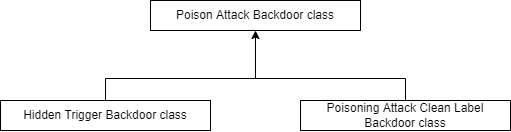
\includegraphics[width=9cm]{pictures/attack_relationship.png}
  \caption{Both attack classes (\textit{PoisoningAttackCleanLabelBackdoor} and \textit{HiddenTriggerBackdoor}) get the backdoor from the \textit{PoisoningAttackBackdoor}}
  \label{fig:relation_risk_ind}
\end{figure}

\subsection{The logging function}

Assigned values of the risk indicators are represented with an optimized logging function, based on the Python logging module. The function waits for two parameters. A message string and the wanted logging level (i.e. INFO or DEBUG). The called log function in the RMF could look like this:
\begin{lstlisting}
  log(f"{variable_name}", 'INFO')
\end{lstlisting}

In order not to depend on the different ML libraries the rmf gets its own functions of the different metrics. That increases the support of different Python libraries for ML risk
measurement.

\subsection{Using the threat model}
\subsection{Evaluation with the measurement construct of ISO 27004}
\subsection{Show the measurement results}
